
\section{Review of MUMPS Library}
\label{subseq:mumps-review}

Originally, MUMPS library was a part of the PARASOL Project. The project was an ESPRIT IV Long Term Research whose main goal was to build and test a portable library for solving large sparse systems of equations on distributed memory systems \cite{PARASOL}. An important aspect of the researh was the strong link between the developers of the sparse solvers and the industrial end users, who provided a range of test problems and evaluated the solvers \cite{MUMPS:description}. Since 2000 MUMPS had continued as an ongoing project and, by the moment of writing, the library have contained almost 5 main releases.\\



It was mentioned in section \ref{subseq:mm-library-choice} that MUMPS is an implementation of the multifrontal method. Hence, MUMPS sequentially performs all three phases: analysis, numerical factorization and solution. The numerical factorization and solution phases were fully described in detail in section \ref{subseq:sparse methods}. It is important to examine the analysis phase of MUMPS library because this phase varies from library to library and plays a significant role on parallel performance.\\


According to the documentation, the MUMPS analysis phases consists of several pre-processing steps:

\begin{enumerate}
  \item Fill-reducing pivot order \label{mumps:analysis-steps:1}
  \item Symbolic factorization \label{mumps:analysis-steps:2}
  \item Scaling \label{mumps:analysis-steps:3}
  \item Amalgamantion \label{mumps:analysis-steps:4}
  \item Mapping \label{mumps:analysis-steps:5}
\end{enumerate}


% Fill-reducing pivot order
\ref{mumps:analysis-steps:1}) To handle both symmetric and unsymmetric cases, MUMPS performs fill-in reordering based on $\boldsymbol{A} + \boldsymbol{A^T}$ sparsity pattern. The library provides numerous sequantial algorithms for reordering such as Approximate Minimum Degree (AMD) \cite{reordering:AMD}, Approximate Minimum Fill (AMF), Approximate Minimum Degree with automatic quasi-dense row detection (QAMD) \cite{reordering:QAMD}, Bottom-up and Top-down Sparse Reordering (PORD) \cite{reordering:PORD}, Nested Dissection coupled with AMD (Scotch) \cite{reordering:SCOTCH}, Multilevel Nested Dissection coupled with Multiple Minimum Degree (METIS) \cite{reordering:METIS}. Additionally, MUMPS can work together with ParMETIS and PT-Scotch which are extensions of METIS and Scotch libraries for parallel execution. MUMPS also provides the user with an automatic choice option where an appropriate reordering algorithm is selected in run-time based on matrix type and size and the number of processors \cite{mumps-manual}.\\


% Symbolic factorization
\ref{mumps:analysis-steps:2}) Sparsity structures of factors $L$ and $U$ are computed during the step, based on permuted matrix $A$ after fill reducing reordering, in order to build the corresponding elimination tree. All computations are performed on a directed graph $G(A)$ associated with the matrix $A$.\\


% Scaling
\ref{mumps:analysis-steps:3}) At this step, matrix $A$ is scaled in such a way to get absolute values of \textit{one} along the main diagonal and \textit{less than one} for all off-diagonal entries. Scaling algorithms are based on sudies described in detail in works \cite{mm:scaling:duff1999design}, \cite{mm:scaling:duff2001algorithms} (for the unsymmetric case) and \cite{mm:scaling:duff2005strategies} (for the symmetric case). This preprocessing step is supposed to improve numerical accuracy and makes all estimations performed during analysis more reliable \cite{mumps-manual}. MUMPS also provides an option to switch off scaling or perform it during the factorization phase.\\



% Amalgamantion
\ref{mumps:analysis-steps:4}) During amalgamantion, sets of columns with the same off-diagonal sparsity pattern are group together to create bigger nodes, also known as supernodes. The process leads to restructuring of the initial elimination tree to an amalgamated tree of supernodes which is also know as the \textit{assembly tree}. The main purpose of that step is to improve efficiency of dense matrix operations. An example of the amalgamantion process is shown in section \ref{subseq:sparse methods}.\\


% Mapping
\ref{mumps:analysis-steps:5}) A host process, chosen by MUMPS, creates a pool of tasks where each task can be either a subtree or type 2 or type 3 node (figure \ref{fig:mumps-task-data-parallelism}). Then each task is mapped by the host among all available processes in such a way to achieve good memory and compute balance.\\

 
Type 1 nodes are grouped in subtrees, according to the algorithm [reference], and each subtree is processed only by one process to avoid the finest granularity, which can cause high communication overheads. \\


In case of type 2 nodes, the host process assigns each node to one process, which is called the master, which holds fully summed rows and columns of the node and perform pivoting and factorization of these rows. During the numerical factorization phase, in run-time, the master process first receives symbolic information which describes the structure of the contribution blocks sent by its children. At the next step, the master collects information concerning the load of all other processes and decides which of them (\textit{slaves}) are going to participate. Then the master informs the chosen slaves that a new task has been allocated for them and sends them the frontal matrix distribution. After that, the slaves communicates the the children of the master process and collects the corresponding numerical elements. The slaves are in charge of all the assembly and computation of the partly summed rows. \\


The root node belongs to the type 3. The host statically assigns the master for the root, as it is in case of type 2 nodes, to hold all the indices describing the structure of the frontal matrix. Before factorization, the structure of the frontal matrix of the root is statically mapped onto a 2D grid of processes using block cyclic distribution. This allows to determine, during the analysis phase, which process an entry of the root is assigned. Hence, the original matrix entries and the part of the contribution blocks can be assembled as soon as they are available. Due to partial pivoting, the master process collects the index information for all delayed variables of its sons, builds the final structure of the root frontal matrix and broadcast the corresponding symbolic information to all slave processes. The slave, in turn, adjust their local data structure. After that numerical factorization can be perform in parallel.\\


It is important to mention that if the size of the root node is less than a certain computer depended parameter, defined by MUMPS, the root node will be treated as the type 2.\\


An illustrative example of process a mapping together with a combination of static and dynamic scheduling is given in figure \ref{fig:mumps:mapping-and-scheduling}.\\


\figpointer{fig:mumps:mapping-and-scheduling}
\begin{figure}[htpb]
  \centering
  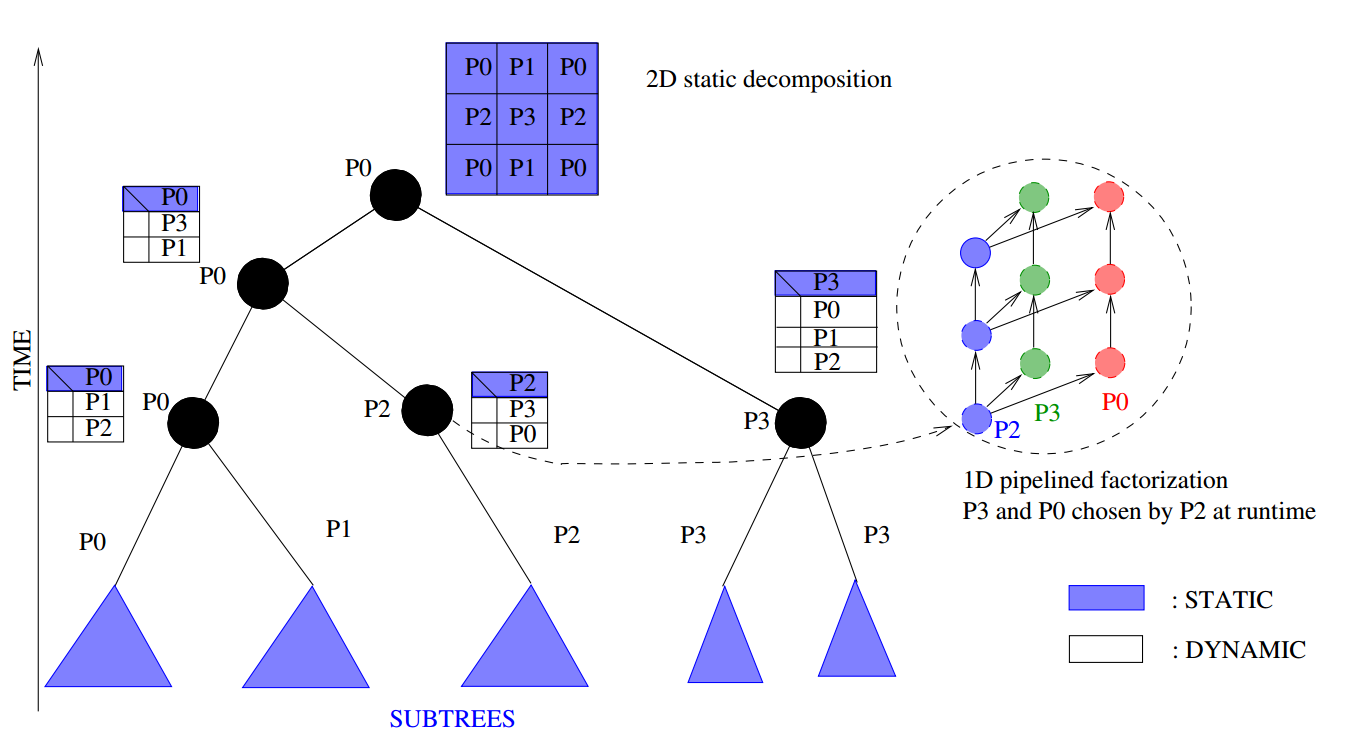
\includegraphics[width=0.85\textwidth]{figures/chapter-2/mumps-task-data-parallelism-2.png}
\caption{MUMPS: static and dynamic scheduling \cite{l2012multifrontal}}
\label{fig:mumps:mapping-and-scheduling}
\end{figure}



Another outstanding feature of MUMPS is treatment of partial pivoting during the numerical factorization phase. To handle this, MUMPS uses threshold pivoting and delayed pivots approaches which are fully described in section \ref{subseq:mm-library-choice} where different implementations of direct sparse solvers are compared.\\


